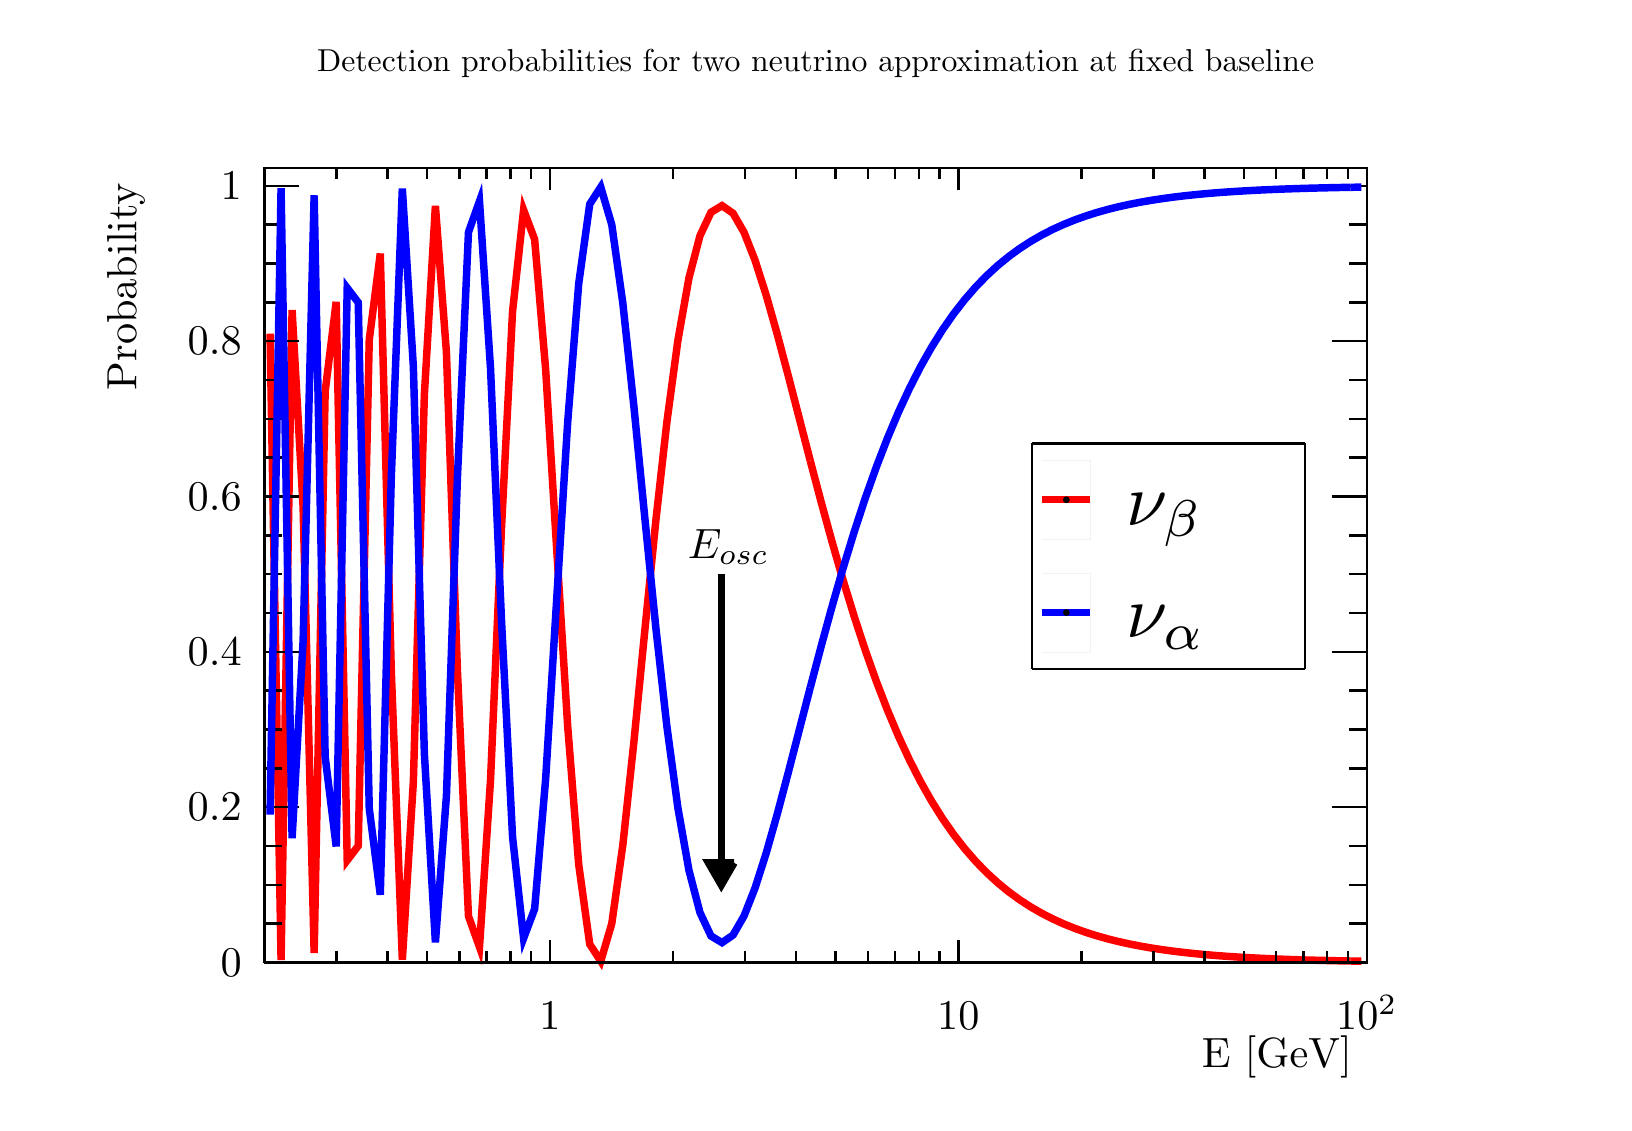
\begin{tikzpicture}
\pgfdeclareplotmark{cross} {
\pgfpathmoveto{\pgfpoint{-0.3\pgfplotmarksize}{\pgfplotmarksize}}
\pgfpathlineto{\pgfpoint{+0.3\pgfplotmarksize}{\pgfplotmarksize}}
\pgfpathlineto{\pgfpoint{+0.3\pgfplotmarksize}{0.3\pgfplotmarksize}}
\pgfpathlineto{\pgfpoint{+1\pgfplotmarksize}{0.3\pgfplotmarksize}}
\pgfpathlineto{\pgfpoint{+1\pgfplotmarksize}{-0.3\pgfplotmarksize}}
\pgfpathlineto{\pgfpoint{+0.3\pgfplotmarksize}{-0.3\pgfplotmarksize}}
\pgfpathlineto{\pgfpoint{+0.3\pgfplotmarksize}{-1.\pgfplotmarksize}}
\pgfpathlineto{\pgfpoint{-0.3\pgfplotmarksize}{-1.\pgfplotmarksize}}
\pgfpathlineto{\pgfpoint{-0.3\pgfplotmarksize}{-0.3\pgfplotmarksize}}
\pgfpathlineto{\pgfpoint{-1.\pgfplotmarksize}{-0.3\pgfplotmarksize}}
\pgfpathlineto{\pgfpoint{-1.\pgfplotmarksize}{0.3\pgfplotmarksize}}
\pgfpathlineto{\pgfpoint{-0.3\pgfplotmarksize}{0.3\pgfplotmarksize}}
\pgfpathclose
\pgfusepathqstroke
}
\pgfdeclareplotmark{cross*} {
\pgfpathmoveto{\pgfpoint{-0.3\pgfplotmarksize}{\pgfplotmarksize}}
\pgfpathlineto{\pgfpoint{+0.3\pgfplotmarksize}{\pgfplotmarksize}}
\pgfpathlineto{\pgfpoint{+0.3\pgfplotmarksize}{0.3\pgfplotmarksize}}
\pgfpathlineto{\pgfpoint{+1\pgfplotmarksize}{0.3\pgfplotmarksize}}
\pgfpathlineto{\pgfpoint{+1\pgfplotmarksize}{-0.3\pgfplotmarksize}}
\pgfpathlineto{\pgfpoint{+0.3\pgfplotmarksize}{-0.3\pgfplotmarksize}}
\pgfpathlineto{\pgfpoint{+0.3\pgfplotmarksize}{-1.\pgfplotmarksize}}
\pgfpathlineto{\pgfpoint{-0.3\pgfplotmarksize}{-1.\pgfplotmarksize}}
\pgfpathlineto{\pgfpoint{-0.3\pgfplotmarksize}{-0.3\pgfplotmarksize}}
\pgfpathlineto{\pgfpoint{-1.\pgfplotmarksize}{-0.3\pgfplotmarksize}}
\pgfpathlineto{\pgfpoint{-1.\pgfplotmarksize}{0.3\pgfplotmarksize}}
\pgfpathlineto{\pgfpoint{-0.3\pgfplotmarksize}{0.3\pgfplotmarksize}}
\pgfpathclose
\pgfusepathqfillstroke
}
\pgfdeclareplotmark{newstar} {
\pgfpathmoveto{\pgfqpoint{0pt}{\pgfplotmarksize}}
\pgfpathlineto{\pgfqpointpolar{44}{0.5\pgfplotmarksize}}
\pgfpathlineto{\pgfqpointpolar{18}{\pgfplotmarksize}}
\pgfpathlineto{\pgfqpointpolar{-20}{0.5\pgfplotmarksize}}
\pgfpathlineto{\pgfqpointpolar{-54}{\pgfplotmarksize}}
\pgfpathlineto{\pgfqpointpolar{-90}{0.5\pgfplotmarksize}}
\pgfpathlineto{\pgfqpointpolar{234}{\pgfplotmarksize}}
\pgfpathlineto{\pgfqpointpolar{198}{0.5\pgfplotmarksize}}
\pgfpathlineto{\pgfqpointpolar{162}{\pgfplotmarksize}}
\pgfpathlineto{\pgfqpointpolar{134}{0.5\pgfplotmarksize}}
\pgfpathclose
\pgfusepathqstroke
}
\pgfdeclareplotmark{newstar*} {
\pgfpathmoveto{\pgfqpoint{0pt}{\pgfplotmarksize}}
\pgfpathlineto{\pgfqpointpolar{44}{0.5\pgfplotmarksize}}
\pgfpathlineto{\pgfqpointpolar{18}{\pgfplotmarksize}}
\pgfpathlineto{\pgfqpointpolar{-20}{0.5\pgfplotmarksize}}
\pgfpathlineto{\pgfqpointpolar{-54}{\pgfplotmarksize}}
\pgfpathlineto{\pgfqpointpolar{-90}{0.5\pgfplotmarksize}}
\pgfpathlineto{\pgfqpointpolar{234}{\pgfplotmarksize}}
\pgfpathlineto{\pgfqpointpolar{198}{0.5\pgfplotmarksize}}
\pgfpathlineto{\pgfqpointpolar{162}{\pgfplotmarksize}}
\pgfpathlineto{\pgfqpointpolar{134}{0.5\pgfplotmarksize}}
\pgfpathclose
\pgfusepathqfillstroke
}
\definecolor{c}{rgb}{1,1,1};
\draw [color=c, fill=c] (0,0) rectangle (20,13.639);
\draw [color=c, fill=c] (3,1.77307) rectangle (17,11.8659);
\definecolor{c}{rgb}{0,0,0};
\draw [c,line width=0.9] (3,1.77307) -- (3,11.8659) -- (17,11.8659) -- (17,1.77307) -- (3,1.77307);
\definecolor{c}{rgb}{1,1,1};
\draw [color=c, fill=c] (3,1.77307) rectangle (17,11.8659);
\definecolor{c}{rgb}{0,0,0};
\draw [c,line width=0.9] (3,1.77307) -- (3,11.8659) -- (17,11.8659) -- (17,1.77307) -- (3,1.77307);
\definecolor{c}{rgb}{1,0,0};
\draw [c,line width=2.7] (3.07109,9.75927) -- (3.21109,1.80536) -- (3.35109,10.0596) -- (3.49109,7.55191) -- (3.63109,1.89456) -- (3.77109,9.02525) -- (3.91109,10.1634) -- (4.05109,3.07134) -- (4.19109,3.25521) -- (4.33109,9.683) -- (4.47109,10.7773)
 -- (4.61109,5.4732) -- (4.75109,1.80887) -- (4.89109,4.06795) -- (5.03109,8.98602) -- (5.17109,11.3824) -- (5.31109,9.52216) -- (5.45109,5.47151) -- (5.59109,2.36234) -- (5.73109,1.96957) -- (5.87109,4.09194) -- (6.01109,7.30398) --
 (6.15109,10.0431) -- (6.29109,11.3303) -- (6.43109,10.958) -- (6.57109,9.30701) -- (6.71109,7.02993) -- (6.85109,4.77427) -- (6.99109,3.01631) -- (7.13109,2.00633) -- (7.27109,1.79026) -- (7.41109,2.26863) -- (7.55109,3.26227) -- (7.69109,4.56761)
 -- (7.83109,5.99492) -- (7.97109,7.3896) -- (8.11109,8.64013) -- (8.25109,9.67701) -- (8.39109,10.4667) -- (8.53109,11.0034) -- (8.67109,11.301) -- (8.81109,11.3853) -- (8.95109,11.2888) -- (9.09109,11.0458) -- (9.23109,10.6898) -- (9.37109,10.2515)
 -- (9.51109,9.75752) -- (9.65109,9.2306) -- (9.79109,8.68917) -- (9.93109,8.1478);
\draw [c,line width=2.7] (9.93109,8.1478) -- (10.0711,7.61764) -- (10.2111,7.10686) -- (10.3511,6.62118) -- (10.4911,6.16427) -- (10.6311,5.73825) -- (10.7711,5.34396) -- (10.9111,4.98132) -- (11.0511,4.64958) -- (11.1911,4.34748) --
 (11.3311,4.07346) -- (11.4711,3.82573) -- (11.6111,3.60243) -- (11.7511,3.40166) -- (11.8911,3.22155) -- (12.0311,3.06028) -- (12.1711,2.91612) -- (12.3111,2.78745) -- (12.4511,2.67274) -- (12.5911,2.57061) -- (12.7311,2.47975) -- (12.8711,2.399) --
 (13.0111,2.32728) -- (13.1511,2.26363) -- (13.2911,2.20718) -- (13.4311,2.15713) -- (13.5711,2.11278) -- (13.7111,2.07349) -- (13.8511,2.0387) -- (13.9911,2.00791) -- (14.1311,1.98066) -- (14.2711,1.95656) -- (14.4111,1.93523) -- (14.5511,1.91637)
 -- (14.6911,1.8997) -- (14.8311,1.88495) -- (14.9711,1.87192) -- (15.1111,1.8604) -- (15.2511,1.85022) -- (15.3911,1.84123) -- (15.5311,1.83328) -- (15.6711,1.82625) -- (15.8111,1.82005) -- (15.9511,1.81456) -- (16.0911,1.80972) -- (16.2311,1.80544)
 -- (16.3711,1.80166) -- (16.5111,1.79832) -- (16.6511,1.79537) -- (16.7911,1.79277);
\draw [c,line width=2.7] (16.7911,1.79277) -- (16.9311,1.79046);
\definecolor{c}{rgb}{0,0,0};
\draw [c,line width=0.9] (3,1.77307) -- (17,1.77307);
\draw [c,line width=0.9] (3.00001,1.91628) -- (3.00001,1.77307);
\draw [c,line width=0.9] (3.91342,1.91628) -- (3.91342,1.77307);
\draw [c,line width=0.9] (4.5615,1.91628) -- (4.5615,1.77307);
\draw [c,line width=0.9] (5.06418,1.91628) -- (5.06418,1.77307);
\draw [c,line width=0.9] (5.47491,1.91628) -- (5.47491,1.77307);
\draw [c,line width=0.9] (5.82217,1.91628) -- (5.82217,1.77307);
\draw [c,line width=0.9] (6.12299,1.91628) -- (6.12299,1.77307);
\draw [c,line width=0.9] (6.38832,1.91628) -- (6.38832,1.77307);
\draw [c,line width=0.9] (6.62568,2.05948) -- (6.62568,1.77307);
\draw [anchor=base] (6.62568,0.92063) node[scale=1.52731, color=c, rotate=0]{1};
\draw [c,line width=0.9] (8.18717,1.91628) -- (8.18717,1.77307);
\draw [c,line width=0.9] (9.10058,1.91628) -- (9.10058,1.77307);
\draw [c,line width=0.9] (9.74866,1.91628) -- (9.74866,1.77307);
\draw [c,line width=0.9] (10.2513,1.91628) -- (10.2513,1.77307);
\draw [c,line width=0.9] (10.6621,1.91628) -- (10.6621,1.77307);
\draw [c,line width=0.9] (11.0093,1.91628) -- (11.0093,1.77307);
\draw [c,line width=0.9] (11.3102,1.91628) -- (11.3102,1.77307);
\draw [c,line width=0.9] (11.5755,1.91628) -- (11.5755,1.77307);
\draw [c,line width=0.9] (11.8128,2.05948) -- (11.8128,1.77307);
\draw [anchor=base] (11.8128,0.92063) node[scale=1.52731, color=c, rotate=0]{10};
\draw [c,line width=0.9] (13.3743,1.91628) -- (13.3743,1.77307);
\draw [c,line width=0.9] (14.2877,1.91628) -- (14.2877,1.77307);
\draw [c,line width=0.9] (14.9358,1.91628) -- (14.9358,1.77307);
\draw [c,line width=0.9] (15.4385,1.91628) -- (15.4385,1.77307);
\draw [c,line width=0.9] (15.8492,1.91628) -- (15.8492,1.77307);
\draw [c,line width=0.9] (16.1965,1.91628) -- (16.1965,1.77307);
\draw [c,line width=0.9] (16.4973,1.91628) -- (16.4973,1.77307);
\draw [c,line width=0.9] (16.7626,1.91628) -- (16.7626,1.77307);
\draw [c,line width=0.9] (17,2.05948) -- (17,1.77307);
\draw [anchor=base] (17,0.92063) node[scale=1.52731, color=c, rotate=0]{$10^{2}$};
\draw [anchor= east] (17,0.572837) node[scale=1.52731, color=c, rotate=0]{E [GeV]};
\draw [c,line width=0.9] (3,11.8659) -- (17,11.8659);
\draw [c,line width=0.9] (3.00001,11.7227) -- (3.00001,11.8659);
\draw [c,line width=0.9] (3.91342,11.7227) -- (3.91342,11.8659);
\draw [c,line width=0.9] (4.5615,11.7227) -- (4.5615,11.8659);
\draw [c,line width=0.9] (5.06418,11.7227) -- (5.06418,11.8659);
\draw [c,line width=0.9] (5.47491,11.7227) -- (5.47491,11.8659);
\draw [c,line width=0.9] (5.82217,11.7227) -- (5.82217,11.8659);
\draw [c,line width=0.9] (6.12299,11.7227) -- (6.12299,11.8659);
\draw [c,line width=0.9] (6.38832,11.7227) -- (6.38832,11.8659);
\draw [c,line width=0.9] (6.62568,11.5795) -- (6.62568,11.8659);
\draw [c,line width=0.9] (8.18717,11.7227) -- (8.18717,11.8659);
\draw [c,line width=0.9] (9.10058,11.7227) -- (9.10058,11.8659);
\draw [c,line width=0.9] (9.74866,11.7227) -- (9.74866,11.8659);
\draw [c,line width=0.9] (10.2513,11.7227) -- (10.2513,11.8659);
\draw [c,line width=0.9] (10.6621,11.7227) -- (10.6621,11.8659);
\draw [c,line width=0.9] (11.0093,11.7227) -- (11.0093,11.8659);
\draw [c,line width=0.9] (11.3102,11.7227) -- (11.3102,11.8659);
\draw [c,line width=0.9] (11.5755,11.7227) -- (11.5755,11.8659);
\draw [c,line width=0.9] (11.8128,11.5795) -- (11.8128,11.8659);
\draw [c,line width=0.9] (13.3743,11.7227) -- (13.3743,11.8659);
\draw [c,line width=0.9] (14.2877,11.7227) -- (14.2877,11.8659);
\draw [c,line width=0.9] (14.9358,11.7227) -- (14.9358,11.8659);
\draw [c,line width=0.9] (15.4385,11.7227) -- (15.4385,11.8659);
\draw [c,line width=0.9] (15.8492,11.7227) -- (15.8492,11.8659);
\draw [c,line width=0.9] (16.1965,11.7227) -- (16.1965,11.8659);
\draw [c,line width=0.9] (16.4973,11.7227) -- (16.4973,11.8659);
\draw [c,line width=0.9] (16.7626,11.7227) -- (16.7626,11.8659);
\draw [c,line width=0.9] (17,11.5795) -- (17,11.8659);
\draw [c,line width=0.9] (3,1.77307) -- (3,11.8659);
\draw [c,line width=0.9] (3.444,1.77307) -- (3,1.77307);
\draw [c,line width=0.9] (3.222,2.26632) -- (3,2.26632);
\draw [c,line width=0.9] (3.222,2.75958) -- (3,2.75958);
\draw [c,line width=0.9] (3.222,3.25284) -- (3,3.25284);
\draw [c,line width=0.9] (3.444,3.74609) -- (3,3.74609);
\draw [c,line width=0.9] (3.222,4.23935) -- (3,4.23935);
\draw [c,line width=0.9] (3.222,4.73261) -- (3,4.73261);
\draw [c,line width=0.9] (3.222,5.22586) -- (3,5.22586);
\draw [c,line width=0.9] (3.444,5.71912) -- (3,5.71912);
\draw [c,line width=0.9] (3.222,6.21238) -- (3,6.21238);
\draw [c,line width=0.9] (3.222,6.70563) -- (3,6.70563);
\draw [c,line width=0.9] (3.222,7.19889) -- (3,7.19889);
\draw [c,line width=0.9] (3.444,7.69215) -- (3,7.69215);
\draw [c,line width=0.9] (3.222,8.1854) -- (3,8.1854);
\draw [c,line width=0.9] (3.222,8.67866) -- (3,8.67866);
\draw [c,line width=0.9] (3.222,9.17192) -- (3,9.17192);
\draw [c,line width=0.9] (3.444,9.66517) -- (3,9.66517);
\draw [c,line width=0.9] (3.222,10.1584) -- (3,10.1584);
\draw [c,line width=0.9] (3.222,10.6517) -- (3,10.6517);
\draw [c,line width=0.9] (3.222,11.1449) -- (3,11.1449);
\draw [c,line width=0.9] (3.444,11.6382) -- (3,11.6382);
\draw [c,line width=0.9] (3.444,11.6382) -- (3,11.6382);
\draw [anchor= east] (2.9,1.77307) node[scale=1.52731, color=c, rotate=0]{0};
\draw [anchor= east] (2.9,3.74609) node[scale=1.52731, color=c, rotate=0]{0.2};
\draw [anchor= east] (2.9,5.71912) node[scale=1.52731, color=c, rotate=0]{0.4};
\draw [anchor= east] (2.9,7.69215) node[scale=1.52731, color=c, rotate=0]{0.6};
\draw [anchor= east] (2.9,9.66517) node[scale=1.52731, color=c, rotate=0]{0.8};
\draw [anchor= east] (2.9,11.6382) node[scale=1.52731, color=c, rotate=0]{1};
\draw [anchor= east] (1.24,11.8659) node[scale=1.52731, color=c, rotate=90]{Probability};
\draw [c,line width=0.9] (17,1.77307) -- (17,11.8659);
\draw [c,line width=0.9] (16.556,1.77307) -- (17,1.77307);
\draw [c,line width=0.9] (16.778,2.26632) -- (17,2.26632);
\draw [c,line width=0.9] (16.778,2.75958) -- (17,2.75958);
\draw [c,line width=0.9] (16.778,3.25284) -- (17,3.25284);
\draw [c,line width=0.9] (16.556,3.74609) -- (17,3.74609);
\draw [c,line width=0.9] (16.778,4.23935) -- (17,4.23935);
\draw [c,line width=0.9] (16.778,4.73261) -- (17,4.73261);
\draw [c,line width=0.9] (16.778,5.22586) -- (17,5.22586);
\draw [c,line width=0.9] (16.556,5.71912) -- (17,5.71912);
\draw [c,line width=0.9] (16.778,6.21238) -- (17,6.21238);
\draw [c,line width=0.9] (16.778,6.70563) -- (17,6.70563);
\draw [c,line width=0.9] (16.778,7.19889) -- (17,7.19889);
\draw [c,line width=0.9] (16.556,7.69215) -- (17,7.69215);
\draw [c,line width=0.9] (16.778,8.1854) -- (17,8.1854);
\draw [c,line width=0.9] (16.778,8.67866) -- (17,8.67866);
\draw [c,line width=0.9] (16.778,9.17192) -- (17,9.17192);
\draw [c,line width=0.9] (16.556,9.66517) -- (17,9.66517);
\draw [c,line width=0.9] (16.778,10.1584) -- (17,10.1584);
\draw [c,line width=0.9] (16.778,10.6517) -- (17,10.6517);
\draw [c,line width=0.9] (16.778,11.1449) -- (17,11.1449);
\draw [c,line width=0.9] (16.556,11.6382) -- (17,11.6382);
\draw [c,line width=0.9] (16.556,11.6382) -- (17,11.6382);
\definecolor{c}{rgb}{0,0,1};
\draw [c,line width=2.7] (3.07109,3.65199) -- (3.21109,11.6059) -- (3.35109,3.35162) -- (3.49109,5.85935) -- (3.63109,11.5167) -- (3.77109,4.38601) -- (3.91109,3.2479) -- (4.05109,10.3399) -- (4.19109,10.1561) -- (4.33109,3.72827) --
 (4.47109,2.63396) -- (4.61109,7.93806) -- (4.75109,11.6024) -- (4.89109,9.34331) -- (5.03109,4.42524) -- (5.17109,2.02885) -- (5.31109,3.8891) -- (5.45109,7.93975) -- (5.59109,11.0489) -- (5.73109,11.4417) -- (5.87109,9.31933) -- (6.01109,6.10728)
 -- (6.15109,3.36819) -- (6.29109,2.08101) -- (6.43109,2.45325) -- (6.57109,4.10426) -- (6.71109,6.38133) -- (6.85109,8.637) -- (6.99109,10.395) -- (7.13109,11.4049) -- (7.27109,11.621) -- (7.41109,11.1426) -- (7.55109,10.149) -- (7.69109,8.84365) --
 (7.83109,7.41634) -- (7.97109,6.02167) -- (8.11109,4.77114) -- (8.25109,3.73425) -- (8.39109,2.94457) -- (8.53109,2.40784) -- (8.67109,2.1103) -- (8.81109,2.02597) -- (8.95109,2.12248) -- (9.09109,2.36544) -- (9.23109,2.72142) -- (9.37109,3.15979)
 -- (9.51109,3.65374) -- (9.65109,4.18066) -- (9.79109,4.7221) -- (9.93109,5.26346);
\draw [c,line width=2.7] (9.93109,5.26346) -- (10.0711,5.79362) -- (10.2111,6.3044) -- (10.3511,6.79009) -- (10.4911,7.24699) -- (10.6311,7.67302) -- (10.7711,8.06731) -- (10.9111,8.42994) -- (11.0511,8.76168) -- (11.1911,9.06378) --
 (11.3311,9.33781) -- (11.4711,9.58554) -- (11.6111,9.80884) -- (11.7511,10.0096) -- (11.8911,10.1897) -- (12.0311,10.351) -- (12.1711,10.4951) -- (12.3111,10.6238) -- (12.4511,10.7385) -- (12.5911,10.8407) -- (12.7311,10.9315) -- (12.8711,11.0123)
 -- (13.0111,11.084) -- (13.1511,11.1476) -- (13.2911,11.2041) -- (13.4311,11.2541) -- (13.5711,11.2985) -- (13.7111,11.3378) -- (13.8511,11.3726) -- (13.9911,11.4034) -- (14.1311,11.4306) -- (14.2711,11.4547) -- (14.4111,11.476) -- (14.5511,11.4949)
 -- (14.6911,11.5116) -- (14.8311,11.5263) -- (14.9711,11.5393) -- (15.1111,11.5509) -- (15.2511,11.561) -- (15.3911,11.57) -- (15.5311,11.578) -- (15.6711,11.585) -- (15.8111,11.5912) -- (15.9511,11.5967) -- (16.0911,11.6015) -- (16.2311,11.6058) --
 (16.3711,11.6096) -- (16.5111,11.6129) -- (16.6511,11.6159) -- (16.7911,11.6185);
\draw [c,line width=2.7] (16.7911,11.6185) -- (16.9311,11.6208);
\definecolor{c}{rgb}{0,0,0};
\draw [c,line width=2.7] (8.80204,6.70563) -- (8.80204,3.03958);
\draw [c, fill=c] (8.96369,3.03958) -- (8.80204,2.75958) -- (8.64038,3.03958);
\draw [c,line width=2.7] (8.96369,3.03958) -- (8.80204,2.75958) -- (8.64038,3.03958) -- (8.96369,3.03958);
\draw [anchor=base west] (8.18716,6.90293) node[scale=1.52731, color=c, rotate=0]{$E_{osc}$};
\definecolor{c}{rgb}{1,1,1};
\draw [color=c, fill=c] (2,12.8206) rectangle (18,13.5708);
\definecolor{c}{rgb}{0,0,0};
\draw (10,13.1957) node[scale=1.14549, color=c, rotate=0]{Detection probabilities for two neutrino approximation at fixed baseline};
\definecolor{c}{rgb}{1,1,1};
\draw [color=c, fill=c] (12.7507,5.50143) rectangle (16.2178,8.36676);
\definecolor{c}{rgb}{0,0,0};
\draw [c,line width=0.9] (12.7507,5.50143) -- (16.2178,5.50143);
\draw [c,line width=0.9] (16.2178,5.50143) -- (16.2178,8.36676);
\draw [c,line width=0.9] (16.2178,8.36676) -- (12.7507,8.36676);
\draw [c,line width=0.9] (12.7507,8.36676) -- (12.7507,5.50143);
\draw [anchor=base west] (13.6175,7.32808) node[scale=2.6728, color=c, rotate=0]{$\nu_{\beta}$};
\definecolor{c}{rgb}{0.95,0.95,0.95};
\draw [c] (12.8807,7.149) -- (13.4875,7.149) -- (13.4875,8.15186) -- (12.8807,8.15186);
\definecolor{c}{rgb}{1,0,0};
\draw [c,line width=2.7] (12.8807,7.65043) -- (13.4875,7.65043);
\definecolor{c}{rgb}{0,0,0};
\foreach \P in {(13.1841,7.65043)}{\draw[mark options={color=c,fill=c},mark size=2.402402pt,mark=*,mark size=1pt] plot coordinates {\P};}
\draw [anchor=base west] (13.6175,5.89542) node[scale=2.6728, color=c, rotate=0]{$\nu_{\alpha}$};
\definecolor{c}{rgb}{0.95,0.95,0.95};
\draw [c] (12.8807,5.71633) -- (13.4875,5.71633) -- (13.4875,6.7192) -- (12.8807,6.7192);
\definecolor{c}{rgb}{0,0,1};
\draw [c,line width=2.7] (12.8807,6.21776) -- (13.4875,6.21776);
\definecolor{c}{rgb}{0,0,0};
\foreach \P in {(13.1841,6.21776)}{\draw[mark options={color=c,fill=c},mark size=2.402402pt,mark=*,mark size=1pt] plot coordinates {\P};}
\end{tikzpicture}
